\documentclass{standalone}
\usepackage{tikz} % Import the tikz package
\usetikzlibrary{automata} % Import library for drawing automata
\usetikzlibrary{positioning} % ...positioning nodes
\usetikzlibrary{arrows} % ...customizing arrows
\tikzset{node distance=2.5cm,
    every state/.style={
        semithick,
        fill=gray!10},
    initial text={},
    double distance=2pt,
    every edge/.style={
        draw,
        ->,>=stealth',
        auto,
        semithick}}
\let\epsilon\varepsilon
\begin{document}
    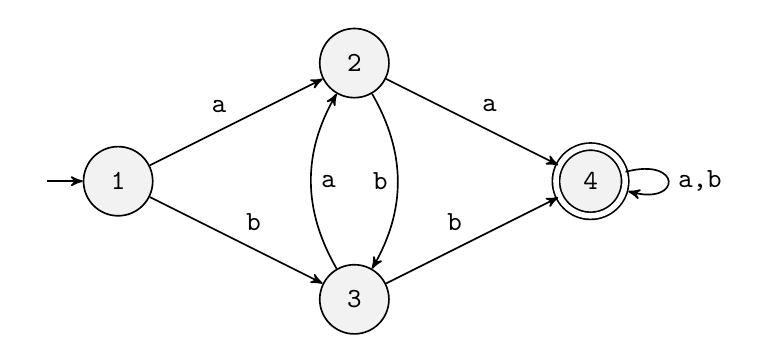
\begin{tikzpicture}
        \node[state,initial] (1) at (0,0) {\tt 1};
        \node[state] (2) at (3,1.5) {\tt 2};
        \node[state] (3) at (3,-1.5) {\tt 3};
        \node[state, accepting] (4) at (6,0) {\tt 4};

        \draw (1) edge[] node {\tt a} (2);
        \draw (1) edge[] node {\tt b} (3);
        
        \draw (2) edge[] node {\tt a} (4);
        \draw (2) edge[bend left,left] node {\tt b} (3);

        \draw (3) edge[bend left,right] node {\tt a} (2);
        \draw (3) edge[] node {\tt b} (4);

        \draw (4) edge[loop right] node {\tt a,b} (4);
    \end{tikzpicture}
\end{document}